%%%%%%%%%%%%%%%%%%%%%%%%%%%%%%%%%%%%%%%%%
% baposter Landscape Poster
% LaTeX Template
% Version 1.0 (11/06/13)
%
% baposter Class Created by:
% Brian Amberg (baposter@brian-amberg.de)
%
% This template has been downloaded from:
% http://www.LaTeXTemplates.com
%
% License:
% CC BY-NC-SA 3.0 (http://creativecommons.org/licenses/by-nc-sa/3.0/)
%
%%%%%%%%%%%%%%%%%%%%%%%%%%%%%%%%%%%%%%%%%

%----------------------------------------------------------------------------------------
%	PACKAGES AND OTHER DOCUMENT CONFIGURATIONS
%----------------------------------------------------------------------------------------

\documentclass[landscape,a0paper,fontscale=0.285]{baposter} % Adjust the font scale/size here

\usepackage{graphicx} % Required for including images
\graphicspath{{figures/}} % Directory in which figures are stored

\usepackage{amsmath} % For typesetting math
\usepackage{amssymb} % Adds new symbols to be used in math mode

\usepackage{booktabs} % Top and bottom rules for tables
\usepackage{enumitem} % Used to reduce itemize/enumerate spacing
\usepackage{palatino} % Use the Palatino font
\usepackage[font=small,labelfont=bf]{caption} % Required for specifying captions to tables and figures
\usepackage{hyperref}
\usepackage{caption}
\usepackage{multicol} % Required for multiple columns
\setlength{\columnsep}{1.5em} % Slightly increase the space between columns
\setlength{\columnseprule}{0mm} % No horizontal rule between columns
\usepackage{multirow}% http://ctan.org/pkg/multirow
\usepackage{hhline}% http://ctan.org/pkg/hhline
\usepackage{tikz} % Required for flow chart
\usepackage{bm}
\usetikzlibrary{shapes,arrows} % Tikz libraries required for the flow chart in the template

\newcommand{\compresslist}{ % Define a command to reduce spacing within itemize/enumerate environments, this is used right after \begin{itemize} or \begin{enumerate}
\setlength{\itemsep}{1pt}
\setlength{\parskip}{0pt}
\setlength{\parsep}{0pt}
}

\definecolor{lightblue}{rgb}{.6,0,0} % Defines the color used for content box headers

\begin{document}

\begin{poster}
{
headerborder=closed, % Adds a border around the header of content boxes
colspacing=1em, % Column spacing
bgColorOne=white, % Background color for the gradient on the left side of the poster
bgColorTwo=white, % Background color for the gradient on the right side of the poster
borderColor=lightblue, % Border color
headerColorOne=white, % Background color for the header in the content boxes (left side)
headerColorTwo=lightblue, % Background color for the header in the content boxes (right side)
headerFontColor=black, % Text color for the header text in the content boxes
boxColorOne=white, % Background color of the content boxes
textborder=roundedleft, % Format of the border around content boxes, can be: none, bars, coils, triangles, rectangle, rounded, roundedsmall, roundedright or faded
eyecatcher=true, % Set to false for ignoring the left logo in the title and move the title left
headerheight=0.1\textheight, % Height of the header
headershape=roundedright, % Specify the rounded corner in the content box headers, can be: rectangle, small-rounded, roundedright, roundedleft or rounded
headerfont=\Large\bf\textsc, % Large, bold and sans serif font in the headers of content boxes
%textfont={\setlength{\parindent}{1.5em}}, % Uncomment for paragraph indentation
linewidth=2pt % Width of the border lines around content boxes
}
%----------------------------------------------------------------------------------------
%	TITLE SECTION 
%----------------------------------------------------------------------------------------
%
{
\includegraphics[height=5em]{usc_logo.png}} % First university/lab logo on the left
{\bf\textsc{\huge High-Resolution Image Inpainting using Multi-Scale Neural Patch Synthesis}\vspace{0.5em}} % Poster title
{\textsc{\{Chao ``Harry'' Yang, Xin Lu, Zhe Lin, Eli Schechtman, Oliver Wang and Hao Li\} \hspace{12pt} \parbox{0.3\textwidth}{\small *University of Southern California\\$^\dagger$Adobe Research}}} % Author names and institution
{
\includegraphics[height=5em]{adobe_logo.jpg}} 
%----------------------------------------------------------------------------------------
%	OBJECTIVES
%----------------------------------------------------------------------------------------

\headerbox{Bad Things Happen}{name=objectives,column=0,span=2, row=0}{
\begin{minipage}[t]{1\linewidth}
\begin{center}
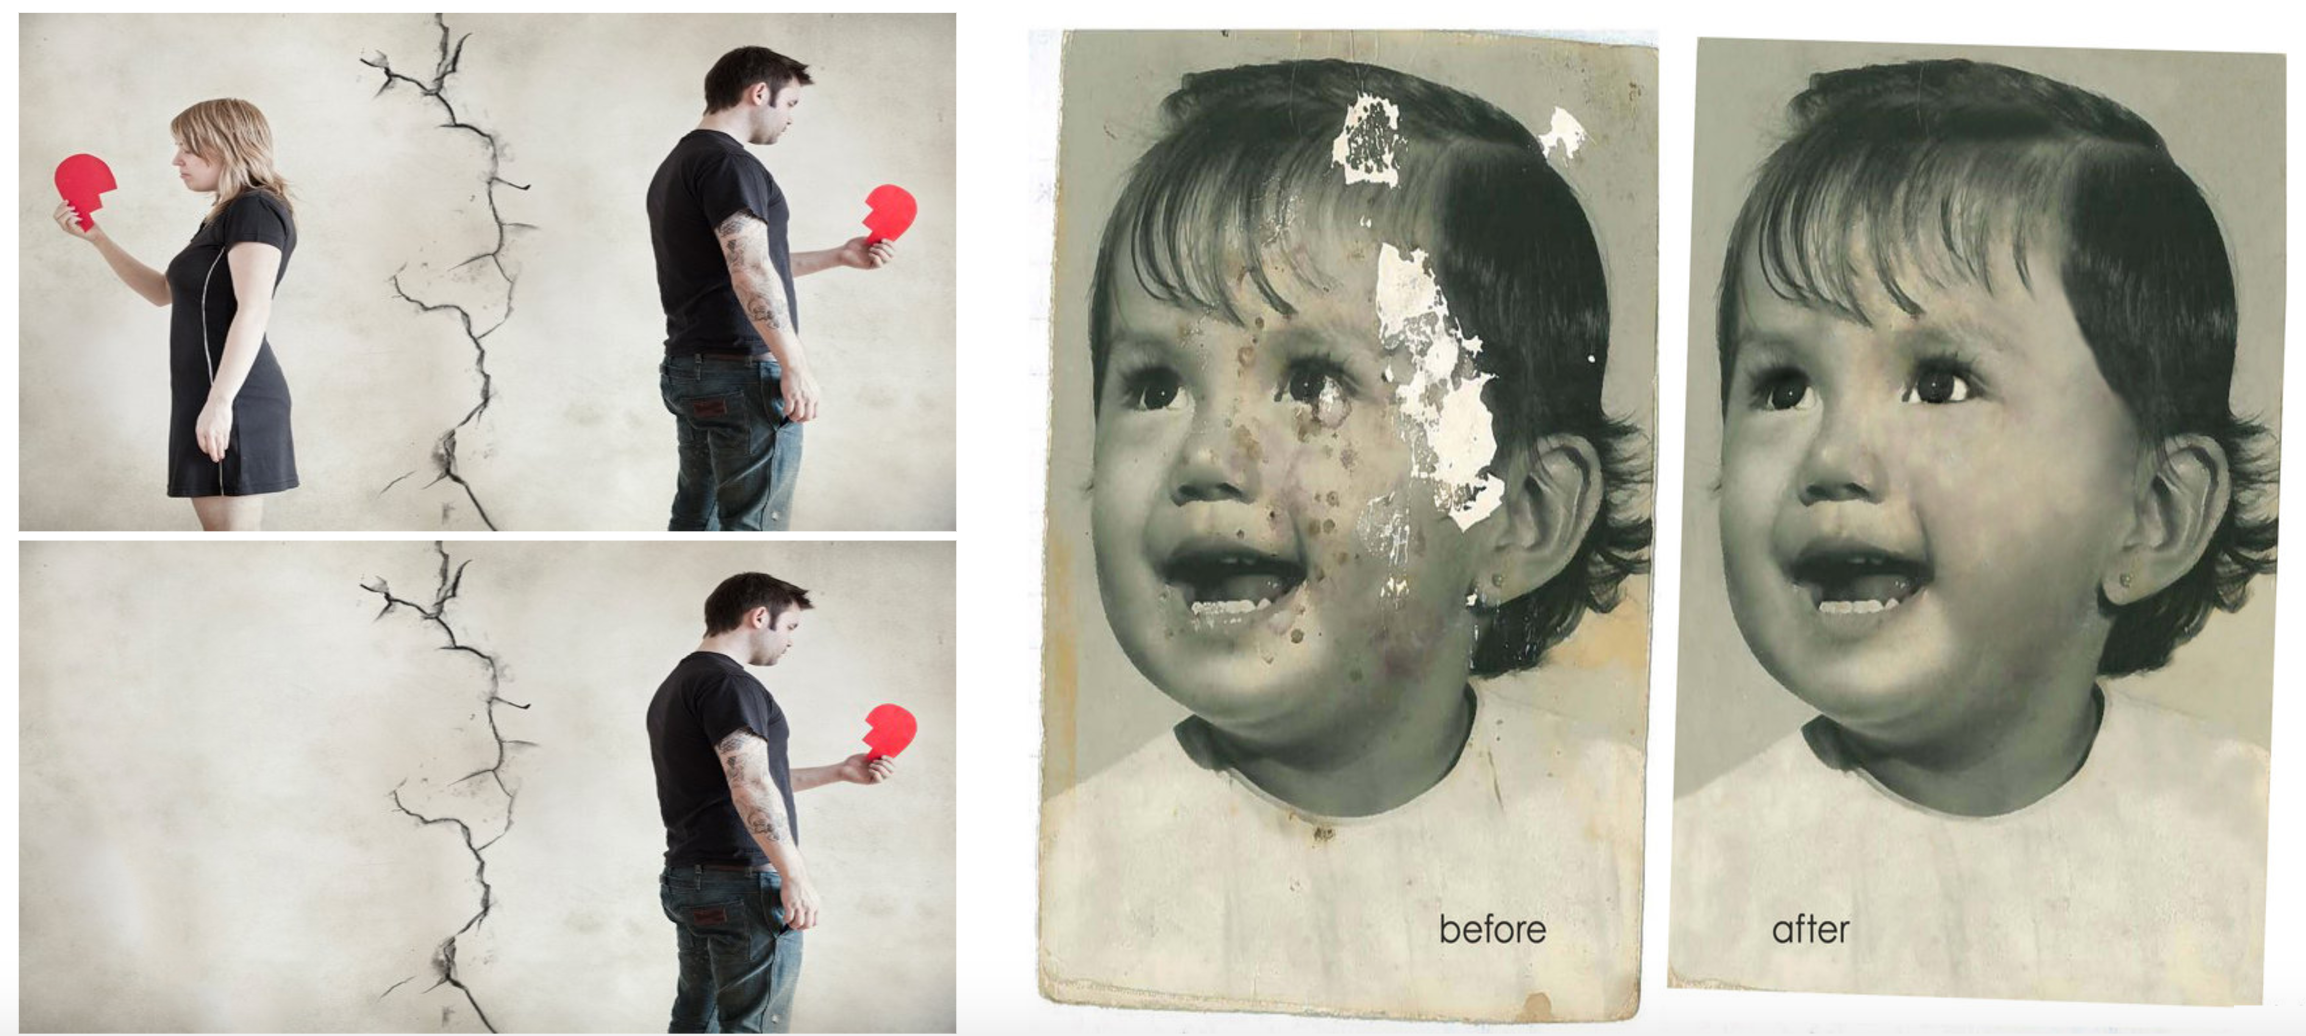
\includegraphics[width=1\columnwidth]{figures/problem.png}
\end{center}
\end{minipage}
Imaging you would like to edit a photo after breaking up, or restore an old picture from damages, we designed a MULTI-SCALE DEEP LEARNING algorithm to help you! We
\begin{itemize}
\item proposed a joint optimization framework that can hallucinates missing image regions by modeling a global content constraint and local texture constraint with convolutional neural networks.
\item further introduced a multi-scale neural patch syn- thesis algorithm for high-resolution image inpainting based on the joint optimization framework.
\end{itemize}
\vspace{0.3em} % When there are two boxes, some whitespace may need to be added if the one on the right has more content
}

%----------------------------------------------------------------------------------------
%	INTRODUCTION
%----------------------------------------------------------------------------------------

\headerbox{The Content and Texture Network}{name=introduction,column=2,span=2, row=0}{
\begin{minipage}{1\linewidth}
\begin{center}
\noindent\textbf{From low-res: the content network}
\end{center}
\begin{minipage}[t]{1\linewidth}
\begin{center}
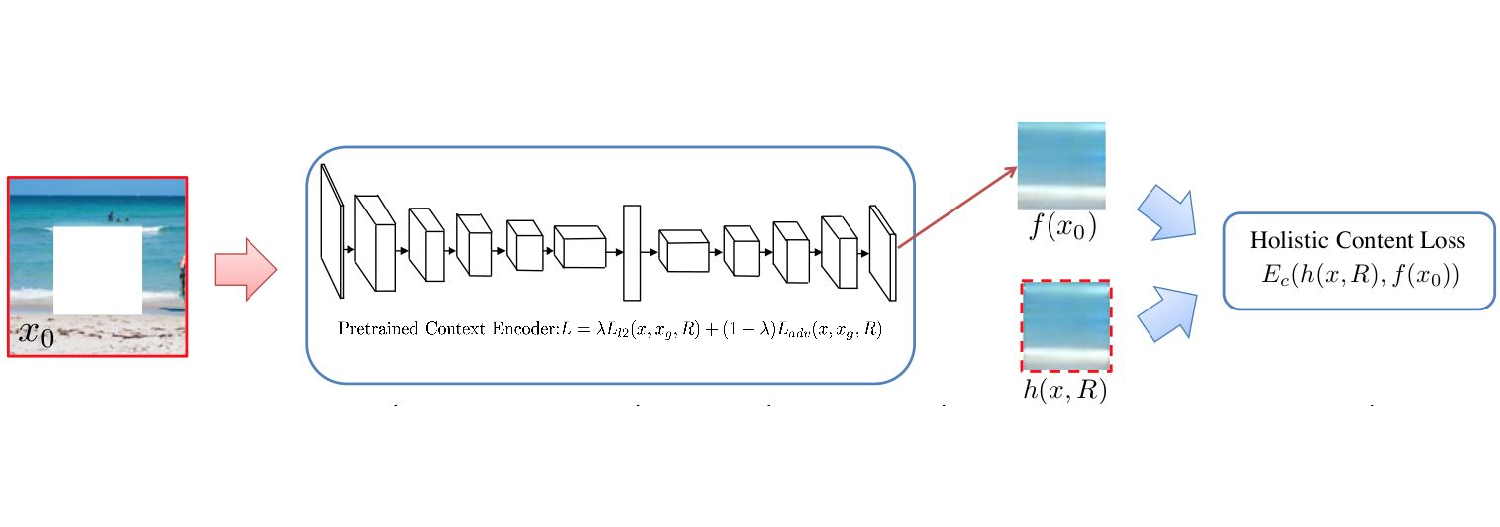
\includegraphics[width=1\columnwidth]{figures/content_network_crop.pdf}
\end{center}
\end{minipage}
\noindent\textbf{To high-res: the texture network}
A typical joint graphical lasso is formulated as the following optimization problem:
\begin{equation}
\min \sum_{k=1}^{K} L({\bm{\Theta}}^{(k)}) + P(\bm{\Theta}) 
\end{equation}
Where $\bm{\Theta}^{(k)} \succ 0$ is the precision matrix $(k=1, \dots ,K)$ and $\bm{\Theta}$ represents the set of $\bm{\Theta}^{(k)}$. The negative log-likelihood $L(\bm{\Theta}^{(k)})$ and the regularization $P(\bm{\Theta})$  are defined as follows.
\begin{equation}
L(\bm{\Theta}^{(k)}) = -\log \det (\bm{\Theta}^{(k)}) + \mathrm{tr}(\mathcal{S}^{(k)}{\bm{\Theta}}^{(k)})
\end{equation}
\begin{equation}
P(\bm{\Theta}) = \lambda_{1}\sum_{k=1}^{K}\| \bm{\Theta}^{(k)}\|_{1} + \lambda_{2}J(\bm{\Theta})
\end{equation}

Here $\lambda_{1}>0$ and $\lambda_{2}>0$ and $J(\bm{\Theta})$ is some penalty function used to encourage similarity (of the structural patterns) among the $K$ classes. In this paper, we focus on group graphical lasso. That is,
\begin{eqnarray}
J(\bm{\Theta}) = 2\sum_{1 \leq i<j\leq p} \sqrt{\sum_{k=1}^{K}(\bm{\Theta}_{i,j}^{(k)})^{2}}
\end{eqnarray}

\end{minipage}

}

%----------------------------------------------------------------------------------------

%----------------------------------------------------------------------------------------
%	CONTACT INFORMATION
%----------------------------------------------------------------------------------------


%----------------------------------------------------------------------------------------
%	MATERIALS AND METHODS
%----------------------------------------------------------------------------------------



\headerbox{Non-uniform Thresholding}{name=method,column=1,span=3, below=introduction}{ % This block's bottom aligns with the bottom of the conclusion block
\begin{minipage}{0.6\linewidth}
Non-uniform thresholding generates a non-uniform feasible partition by thresholding the $K$ empirical covariance matrices separately. In a non-uniform partition, two variables of the same group in one class may belong to different groups in another class. Figure \ref{illustrate_non_uniform} shows an example of non-uniform partition. In this example, all the matrix elements in white color are set to 0 by non-uniform thresholding. Except the white color, each of the other colors indicates one group. The $7^{\text{th}}$ and $9^{\text{th}}$ variables belong to the same group in the left matrix, but not in the right matrix. Similarly, the $3^{\text{rd}}$ and $4^{\text{th}}$ variables belong to the same group in the right matrix, but not in the left matrix.\\
\vspace{-30pt}
\begin{center}
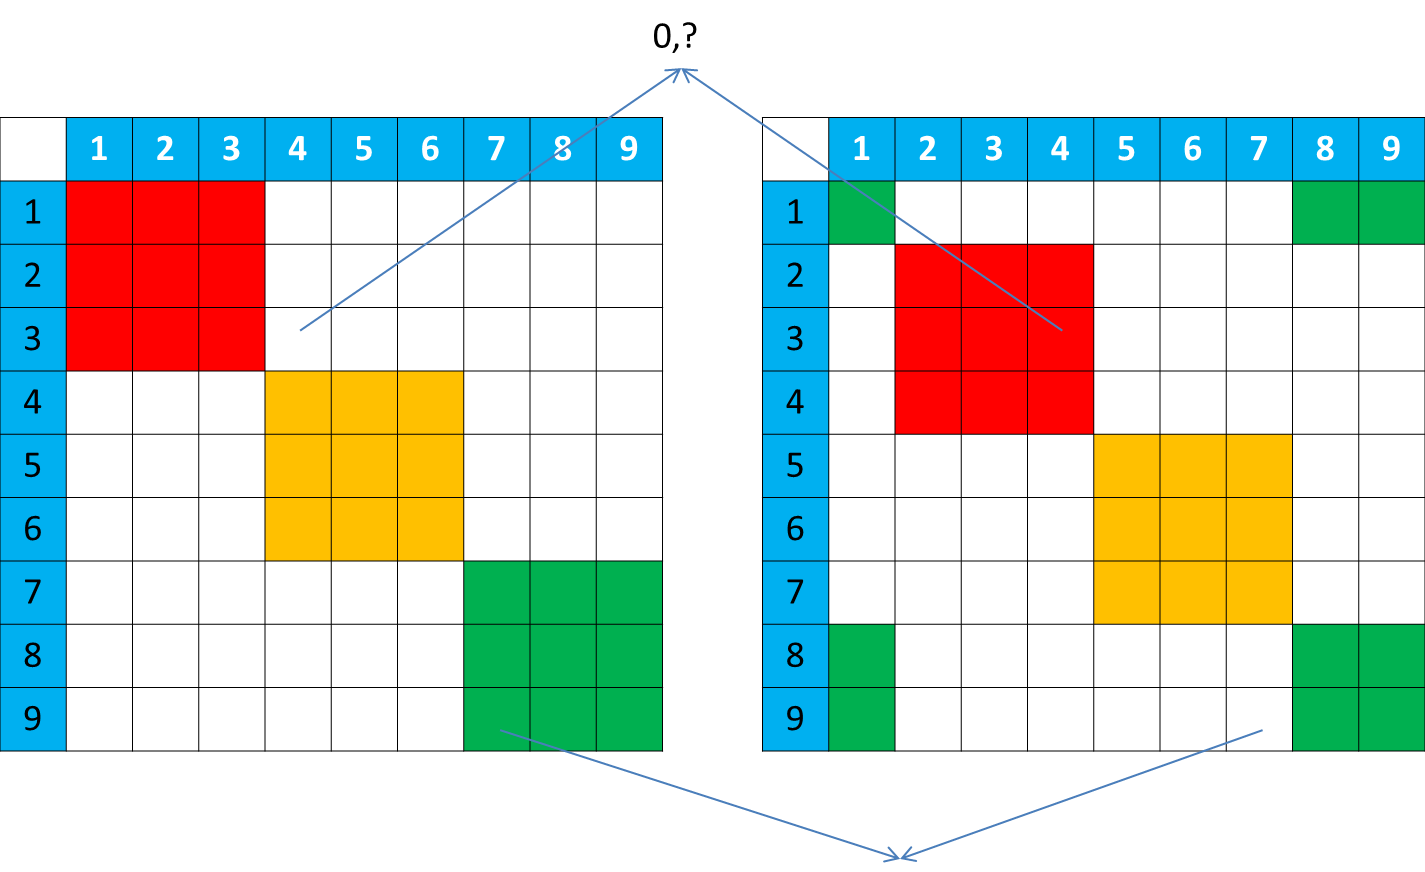
\includegraphics[width=.5\columnwidth]{figures/non_uniform.png}
\end{center}
\end{minipage}
\begin{minipage}[t]{0.35\linewidth}
\vspace{-110pt}
\begin{center}
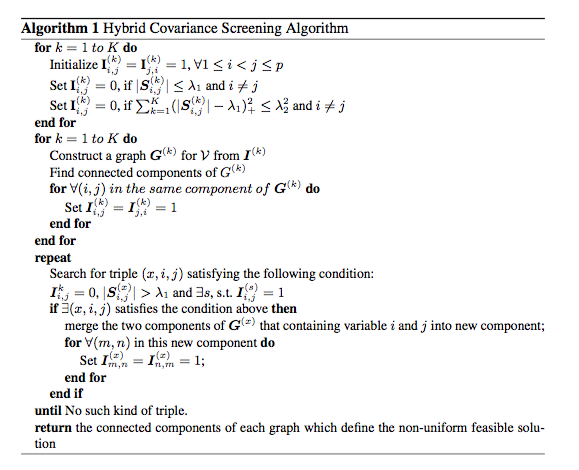
\includegraphics[width=1\columnwidth]{figures/screenshot.png}
\end{center}

\end{minipage}

}


\headerbox{Supplemental and Code}{name=method2,column=1, span=3, below=method}{ % This block's bottom aligns with the bottom of the conclusion block
Code is available at \href{www.harryyang.xyz}www.harryyang.xyz
}

\headerbox{Experiments}{name=method,column=0, below=objectives, bottomaligned=method2}{ % This block's bottom aligns with the bottom of the conclusion block
\begin{itemize}
\item Synthetic data
\vspace{-10pt}
\begin{center}
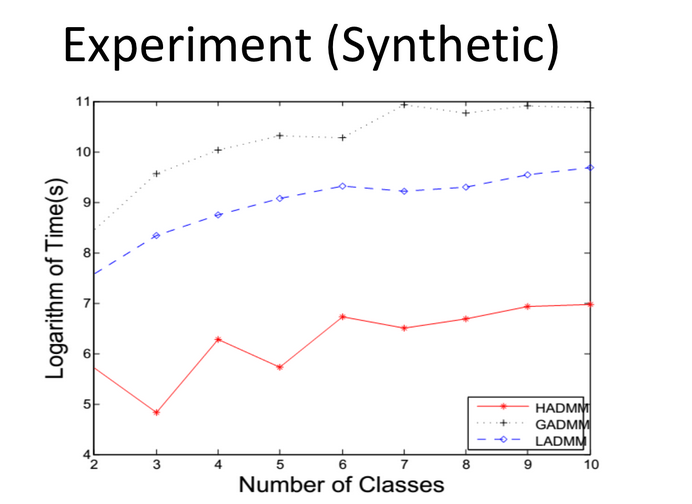
\includegraphics[width=.8\columnwidth]{figures/synthetic.png}
\end{center}
\item Real data
\vspace{-10pt}
\begin{center}
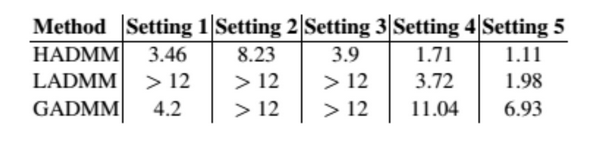
\includegraphics[width=.8\columnwidth]{figures/real.png}
\end{center}
\end{itemize}

}

%----------------------------------------------------------------------------------------
%	RESULTS 2
%----------------------------------------------------------------------------------------



%----------------------------------------------------------------------------------------

\end{poster}

\end{document}